
\renewcommand{\arraystretch}{2}
\renewcommand{\figurename}{Figure}
\chapter{Literature Analysis and State of Art}
\label{chapter:literarure}

\newenvironment{literature}
{\quote\itshape}
{\endquote}

\begin{literature}
This chapter delves into the definition and categorization of weapons, while also elucidating the concept and significance of \ac{cctv}. Deep learning approaches and algorithms employed for this purpose are thoroughly analyzed. Additionally, the contributions of other authors in this field are dissected, offering a comprehensive review of their methodologies and findings. A significant portion of this chapter is dedicated to examining the datasets used by these scholars, highlighting their relevance, comprehensiveness, and potential limitations in the context of real-time weapon detection.
\end{literature}

\section{Context}
\subsection{Weapons}
The Cambridge Dictionary\footnote{https://dictionary.cambridge.org/dictionary/english/weapon} defines a weapon as "any object used in fighting or war, such as a gun, bomb, knife, etc.". This definition suggests that a weapon encompasses any tool or instrument intended to inflict damage or harm, whether on living beings, structures, or systems. Weapons have diverse applications, ranging from hunting and self-defense to warfare. However, their fundamental purpose remains unchanged: they amplify the user's ability to exert force, in either an offensive or defensive capacity.

Weapons can be categorized based on various criteria, including their range, mechanism, or intended use. However, this study will primarily focus on two categories: firearms and melee weapons.

Melee weapons are close-combat instruments that require the user to be in direct proximity to their target, like swords, daggers, maces, and clubs.

Firearms are a subset of ranged weapons that discharge projectiles powered by rapidly expanding high-pressure gas from chemical reactions. They can be further categorized into:
\begin{itemize}
    \item Handguns: Small, handheld firearms like pistols and revolvers.
    \item Rifles: Designed for accuracy, rifles have a longer barrel and are often used in situations requiring precision.
    \item Shotguns: These fire shells that contain multiple pellets, making them effective at close range.
    \item Automatic and Semi-Automatic: Automatic firearms continuously fire bullets as long as the trigger is pressed, while semi-automatics require a trigger pull for each shot.
\end{itemize}

\begin{figure}[h]
    \centering
    \begin{minipage}{0.45\textwidth}
        \centering
        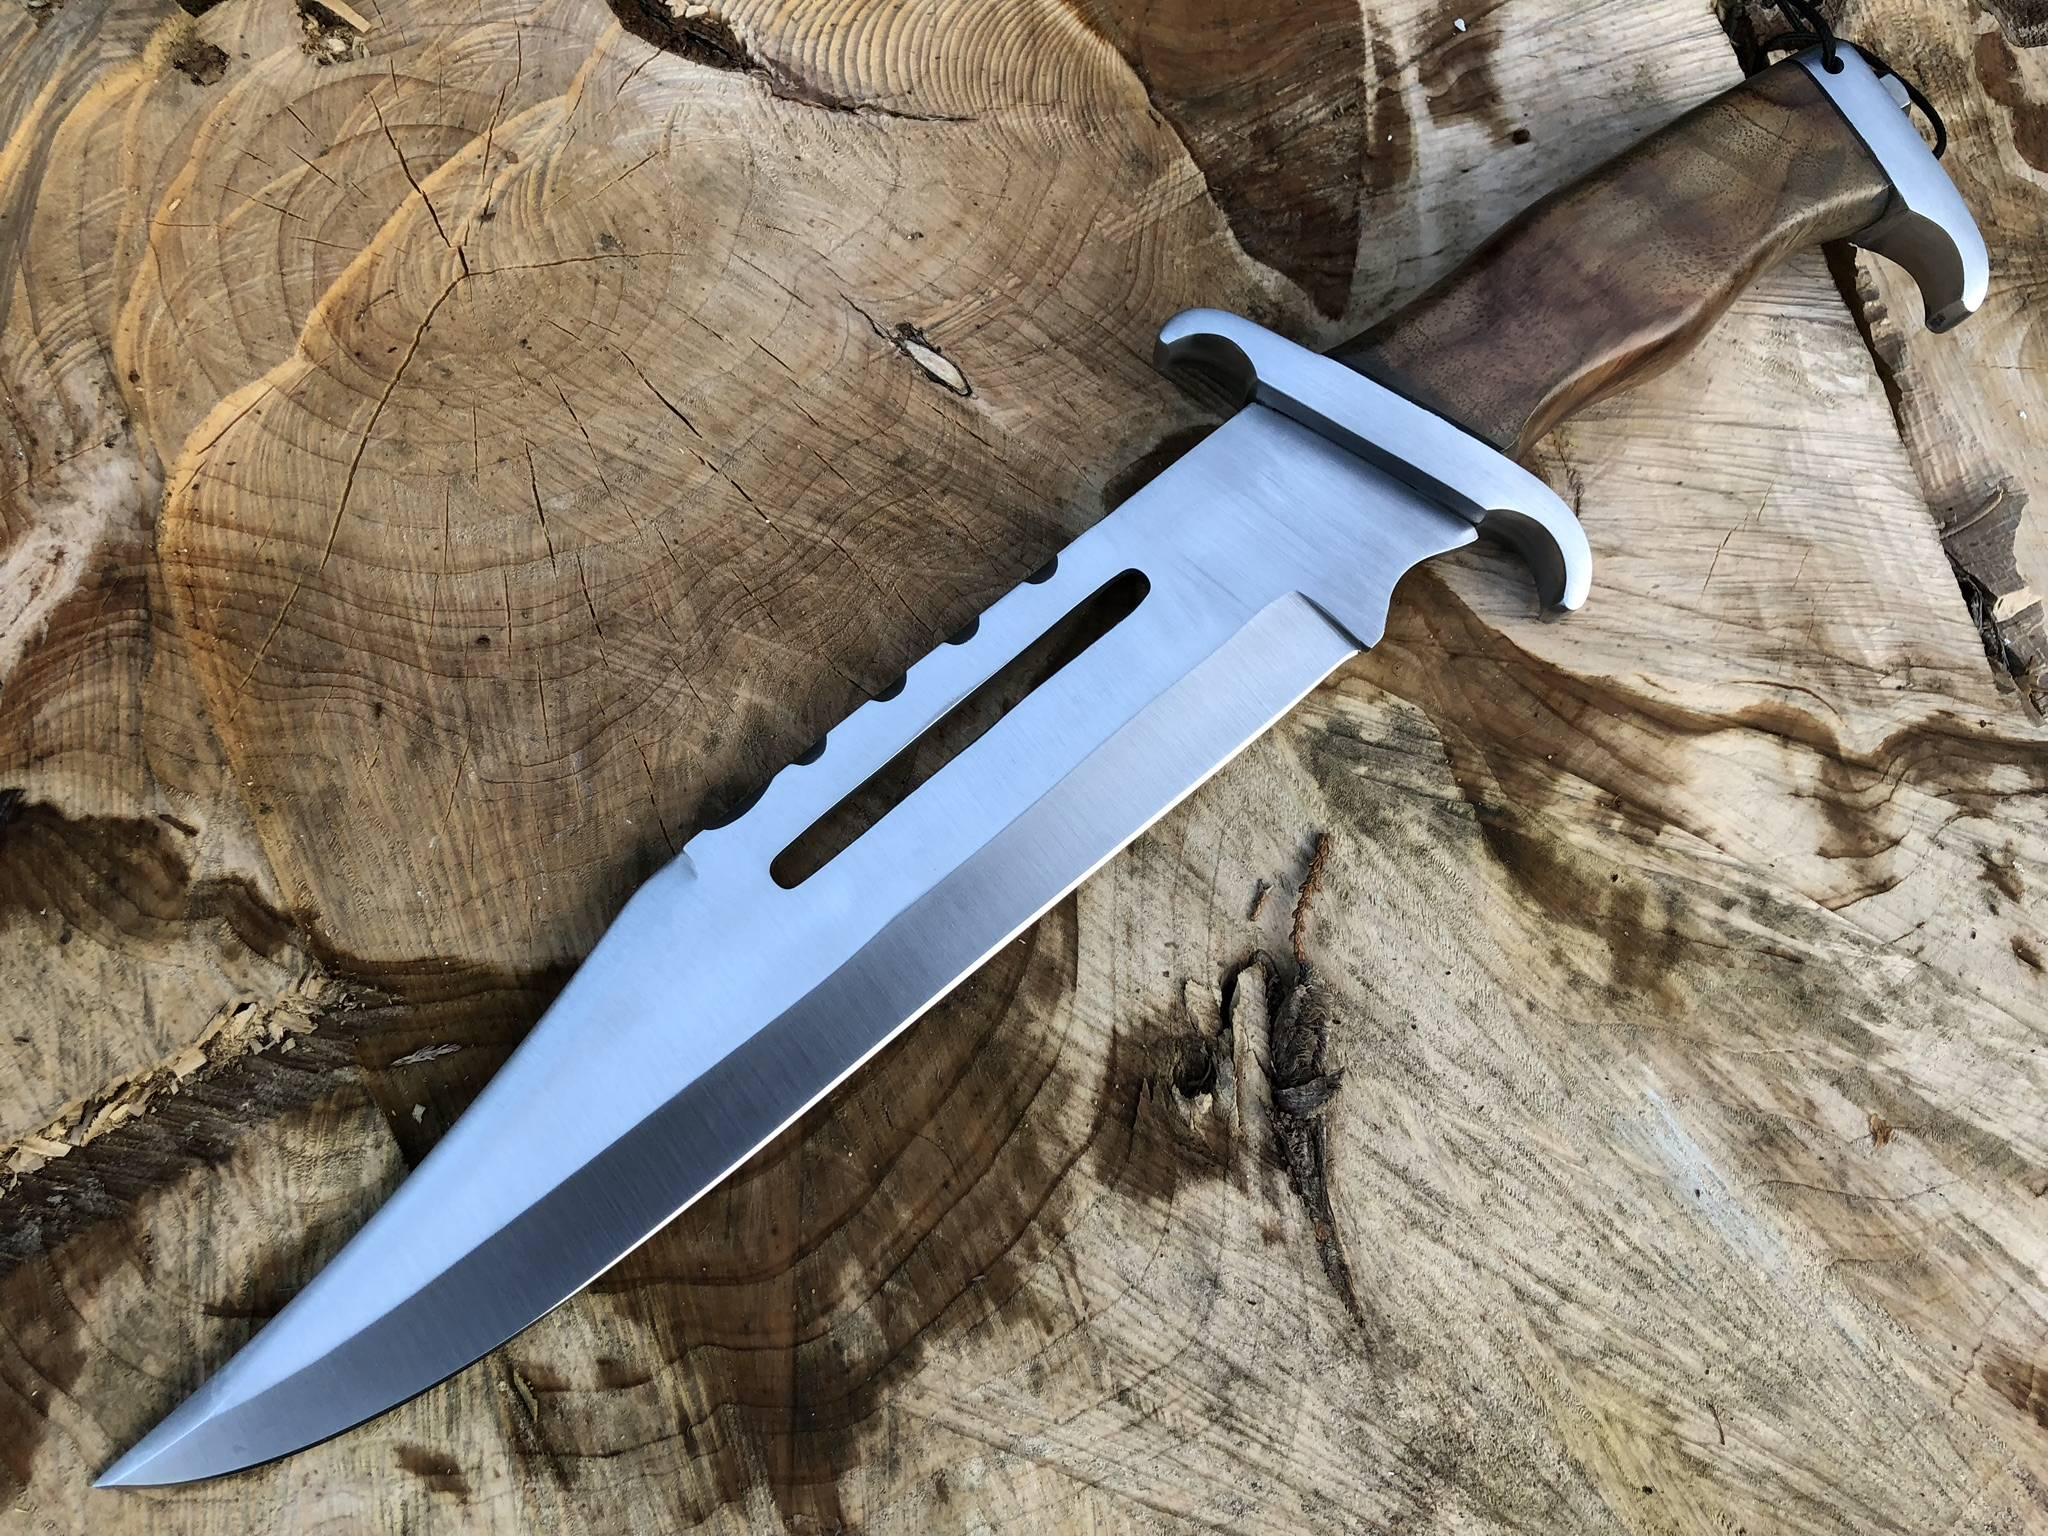
\includegraphics[width=1\linewidth]{figs/knife.jpg}
        \caption{Knife Example}
        \label{fig:first_image}
    \end{minipage}\hfill
    \begin{minipage}{0.48\textwidth}
        \centering
        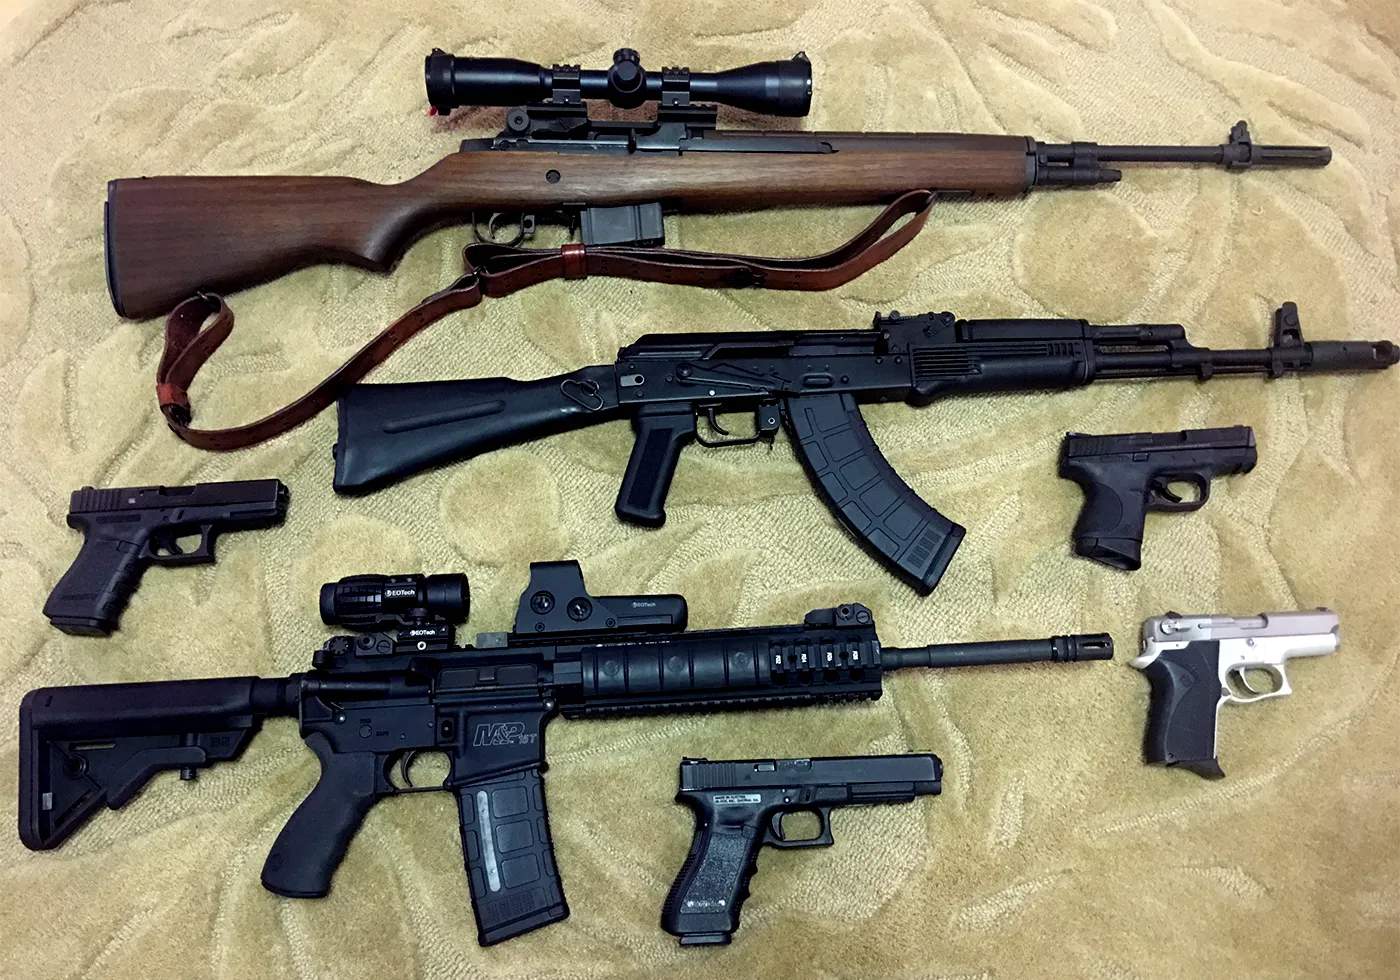
\includegraphics[width=1\linewidth]{figs/firearm.png}
        \caption{Different Firearms Example}
        \label{fig:second_image}
    \end{minipage}
\end{figure}

\subsection{\ac{cctv}}
\ac{cctv} refers to a video surveillance system comprising strategically positioned cameras in various locations. These cameras capture footage, which is then transmitted to monitors for both real-time observation and later playback.

The primary goal of a \ac{cctv} system is to enhance area security through persistent surveillance of key areas. This is highly beneficial for large spaces or sites containing valuable or sensitive items. Besides recording, \ac{cctv} can issue alerts for detected motion, especially during off-hours in vacant business premises. These alerts are crucial for quickly informing authorities about possible security threats.

Additionally, \ac{cctv} systems are not only instrumental in monitoring activities during both operational and non-operational hours but also serve as crucial tools in identifying suspects in criminal activities.

\begin{figure}[h]
    \centering
    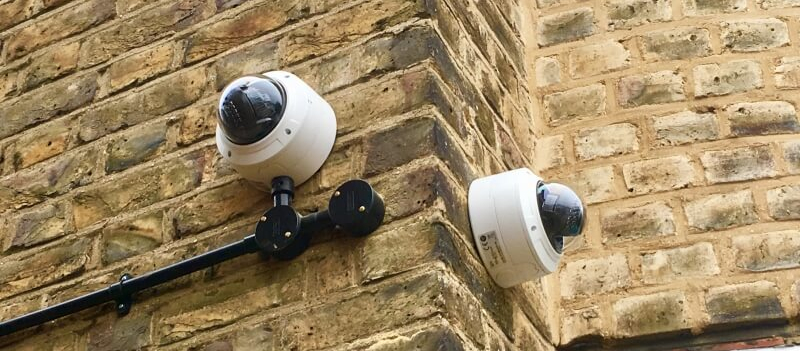
\includegraphics[width=0.45\textwidth]{figs/cctv.jpg}
    \hfill
    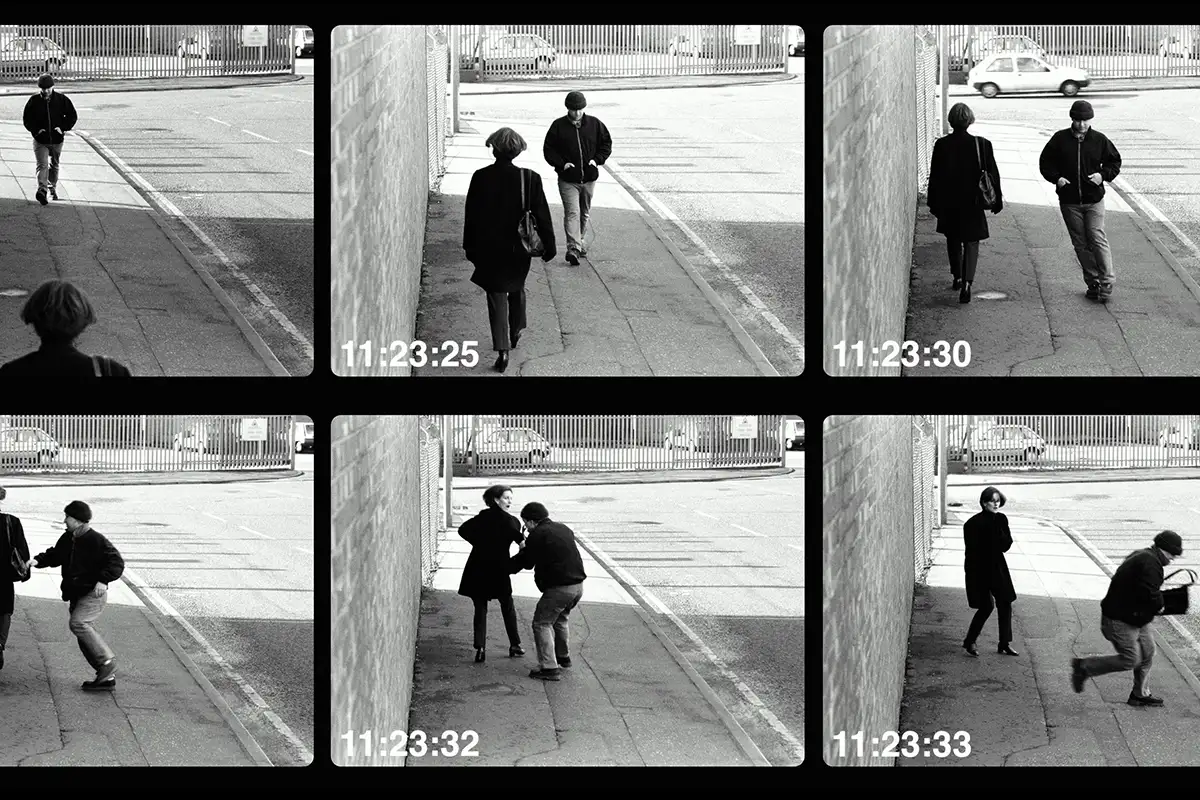
\includegraphics[width=0.45\textwidth]{figs/cctv-footage.png}
    \caption{\ac{cctv} Cameras (Left Image) and \ac{cctv} Footage Samples (Right Image)}
    \label{fig:cctv-and-footage}
\end{figure}


\section{Object Detection}
\subsection{General Concepts}
Object detection stands as a vital component in the realm of computer vision. \selectlanguage{english}\citet{rfc2} describe its goal as "to determine where objects are located in a given image (object localization) and which category each object belongs to (object classification)", undertaking the dual challenge of not only locating an object within the visual frame, creating a bounding box around it, but also determining its category. \selectlanguage{english}\citet{rfc9} further reinforce this stating "Object detection is a fusion of object location and object classification task".

\begin{figure}[h]
    \centering 
    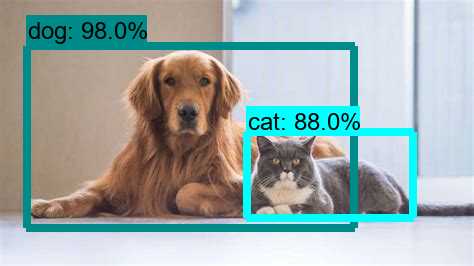
\includegraphics[width=0.5\textwidth]{figs/object-detection.png} 
    \caption{Object Detection Image~\cite{rfc15}}
    \label{fig:object-detection}
\end{figure}

Object detection entails the identification of objects within images and videos. The process of recognizing these objects is fundamentally rooted in the training of object detection models. This crucial training phase involves several key steps:
\begin{itemize}
    \item \textbf{Data Collection}: Gathering a diverse set of images, each showcasing the object in a variety of contexts, including different backgrounds and angles.
    \item \textbf{Labeling}: Annotating each image with labels to show where the object is and confirming its presence
    \item \textbf{Feature Learning}: The neural network learns the object's unique features (like shape, color, texture, patterns) from these labeled images.
    \item \textbf{Generalization}: The ultimate goal of this training is to enable the neural network to not just recognize the object in the training images, but to generalize this knowledge. This allows the model to accurately identify and locate the object in new, unseen images.
\end{itemize} 

The 2014 milestone, Figure \ref{fig:stage-detectors}, marks a pivotal before-and-after in \ac{ai} applications \selectlanguage{english}\cite{rfc22}. Before, the field predominantly utilized traditional methods for tasks like object detection. These methods involved a multi-step process beginning with the selection of regions in images, which was often inefficient and computationally expensive due to the use of techniques like multi-scale sliding windows. Following this, feature extraction methods such as HOG, Haar-like, and SIFT were employed, but these struggled with variability in backgrounds and lighting conditions. The final step, classification, relied on algorithms like Adaboost, but these traditional techniques frequently fell short in terms of accuracy and efficiency \selectlanguage{english}\cite{rfc9}.

After 2014, the landscape of \ac{ai} research underwent a significant transformation with the advent of deep learning-based methods. These new techniques, including Faster RCNN, SSD, and YOLO, revolutionized object detection by automatically learning feature representations from data. This shift not only addressed the limitations of the traditional methods, such as high computational costs and inadequate feature representation, but also led to substantial improvements in both the accuracy and efficiency of object detection processes.

\begin{figure}[h]
    \centering 
    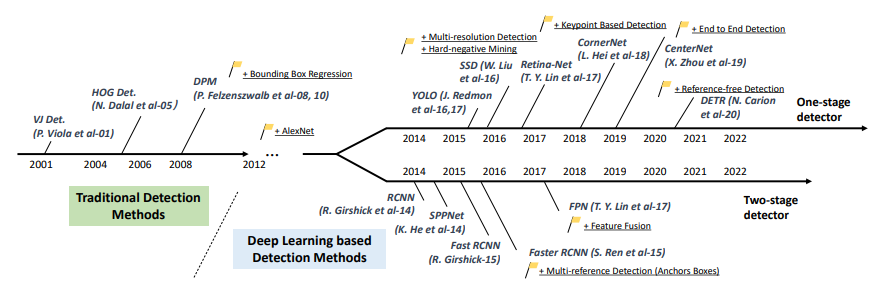
\includegraphics[width=0.9\textwidth]{figs/roadmap-stage.png} 
    \caption{Object Detection Roadmap~\cite{rfc22}}
    \label{fig:stage-detectors}
\end{figure}

There are two primary methodologies, Figure \ref{fig:stage-detectors}, employed for identifying and classifying objects. These methodologies differ significantly in their operational approach and performance characteristics.

Firstly, there is the \textbf{two-stage} detection process. This operate in a sequential two-phase process. The process involves two key steps: "(i) use a Region Proposal Network to generate regions of interests in the first stage and (ii) send the region proposals down the pipeline for object classification and bounding-box regression"\selectlanguage{english}\cite{rfc21}. The two-stage framework ensures high accuracy but at the cost of speed.

Conversely, \textbf{one-stage} detectors treat object detection as a simple regression problem, directly analyzing the image to determine class probabilities and bounding box coordinates. This approach is faster but generally achieves lower accuracy rates compared to two-stage detectors \selectlanguage{english}\cite{rfc23}.

In the field of object detection a variety of metrics are employed to evaluate the performance of detection models. These metrics play a crucial role in both training and testing stages, optimizing classifiers, and measuring their efficiency. 

Precision is calculated as the percentage of correctly identified objects (true positives) among all detections (true and false positives). High precision indicates a low rate of false positives. Recall assesses the model's ability to detect all relevant objects in the dataset. It is the percentage of correctly detected objects (true positives) among all actual objects (sum of true positives and false negatives). High recall implies that the model is effective in identifying most of the relevant objects \selectlanguage{english}\cite{rfc25}.

The \ac{ap} metric integrates precision and recall at different confidence thresholds. It addresses the trade-off between precision and recall, considering detections above a confidence level. \ac{ap} is calculated based on the area under the precision-recall curve \selectlanguage{english}\cite{rfc25}. \ac{map} averages the \ac{ap} across all classes within a database, crucial for assessing multi-class detector performance \selectlanguage{english}\cite{rfc24}. 

F1 score is used to estimate the balance between recall and precision. It is particularly valuable in situations where there is an imbalanced class distribution, as it provides a single metric that combines both precision and recall. Is defined as the harmonic mean\footnote{type of average that gives equal weight to both precision and recall, unlike the arithmetic mean which can be disproportionately influenced by high values of one metric over the other} of precision and recall, \ref{eq:f1score}. 

\begin{equation}
    F1 \text{ score} = 2 \times \frac{\text{Precision} \times \text{Recall}}{\text{Precision} + \text{Recall}}
    \label{eq:f1score}
\end{equation}
    
A high F1 score indicates both high precision and high recall. This metric is particularly useful in the context of binary classifiers on unevenly distributed datasets, where it provides a more balanced view of a model's performance compared to using precision or recall alone \selectlanguage{english}\cite{rfc9}.

\ac{iou} measures the overlap between the predicted \ac{bb} and the ground truth \ac{bb}, Figure \ref{fig:iou}. It's calculated as the ratio of the intersection area to the union area of these BBs. The resulting \ac{iou} value ranges between 0 and 1, with values closer to 1 indicating more accurate detection. "The IoU, based on the Jaccard Index, measures the overlap between the predicted bounding box and the ground-truth bounding box." \selectlanguage{english}\cite{rfc24}.

\begin{figure}[h]
    \centering 
    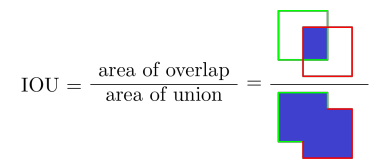
\includegraphics[width=0.5\textwidth]{figs/iou.png} 
    \caption{Intersection over Union \selectlanguage{english}\cite{rfc25}}
    \label{fig:iou}
\end{figure}

\subsection{Algorithms and Techniques Reviews}
This section analyzes current object detection algorithms and methodologies, drawing on a range of studies and innovations from various online repositories and databases. It focuses on selected reviews\footnote{comprehensive overview or evaluation of existing literature on a particular topic} that detail their development, methodologies, outcomes, and contributions to the advancement of object detection. This analysis provides insights into the evolution of object detection techniques from their inception to modern applications.

\selectlanguage{english}\citet{rfc2} delve into the evolution of detection methods, offering a comprehensive review of deep learning-based object detection frameworks. The review starts with a historical overview of deep learning, highlighting the role of CNN\footnote{Convolutional Neural Networks}. The focus then shifts to generic object detection architectures, discussing modifications and strategies to enhance detection performance. Through experimental analyses, various methods for detection tasks are compared, and insightful conclusions are drawn.

\selectlanguage{english}\citet{rfc8} provide a comprehensive review of image processing techniques, emphasizing machine learning applications in visual interpretation. The study begins by highlighting the foundational aspects of computational vision, particularly the significance of array-based media computation in the digital era. It then examines key image processing algorithms, including Single Shot Detection (SSD), Faster Region-based Convolutional Neural Networks (Faster R-CNN), and You Only Look Once (YOLO), detailing their architecture, methodologies, and distinguishing features. The researchers conduct systematic experiments using datasets like Microsoft COCO~\cite{rfc16}, comparing these algorithms to elucidate their respective strengths and limitations.

\selectlanguage{english}\citet{rfc9} emphasize the intricacies of computer vision in their review, highlighting the significant impact of Deep Convolutional Neural Networks (DCNNs). Their study spans various applications, from video processing to speech recognition, with a particular focus on object detection's importance in areas like transportation and security. They detail crucial evaluation metrics, especially Average Precision (AP), for assessing detection effectiveness. Notably, they mark the pivotal shift to deep learning techniques post-2014, analyzing frameworks like SSD and YOLO. By comparing these newer methods with traditional ones and evaluating their performance on datasets like PASCAL VOC~\cite{rfc27} and MS COCO~\cite{rfc16}, they offer insights into the dynamic field of object detection.

\selectlanguage{english}\citet{rfc10} present an in-depth review of deep learning (DL), focusing on its essential concepts, CNN architectures, challenges, and varied applications. The paper initially recognizes DL's increasing prominence in machine learning, often hailed as the 'Gold Standard.' Emphasizing DL's efficiency in processing large datasets, surpassing traditional methods, the authors delve into detailed CNN architectures and their operational principles. They also explore both computational and conceptual challenges in DL. The review further highlights the diverse applications of DL, showcasing its often superior, sometimes human-competitive, performance.

\section{Related Work}
In the pursuit of a deeper understanding and improvement in weapon detection, numerous pivotal studies have emerged, highlighting various techniques, methodologies, and datasets. This section presents a thorough overview of these significant contributions, organizing the discussion into three core subsections: research methods, other author's articles, and datasets.

The first segment delves into the research methodologies where the process employed for locating and selecting relevant literature is detailed. Given the extensive available publications, a meticulous filtering process was employed to choose articles that are critically relevant to weapon detection.

Transitioning to the core of this section, a thorough analysis of the selected articles\footnote{detailed written discourse on a specific subject} is conducted. This part aims to offer an in-depth understanding by meticulously examining the techniques and frameworks proposed by various researchers.

Finally, the attention shifts to the datasets\footnote{collection of related data points, often organized in tables, arrays, or other structures.}. This subsection provides an elaborate overview of the datasets used in weapon detection research, exploring their origins, the methodologies applied for their collection, and highlighting their unique characteristics.

\subsection{Research Method}
This section conducts an in-depth review of pivotal studies in weapon detection, organizing the examination into three focused areas: research methodologies, literature from other authors, and relevant datasets. The breadth and diversity of articles across multiple disciplines required a selective approach. Using specific keywords in Scopus ("deep" AND "learning" AND "real" AND "time" AND "weapon" AND "detection"), 70 records were initially retrieved. Through a rigorous selection process, 8 articles were identified as highly relevant to the study's theme, Figure \ref{fig:scopus_query}.
\begin{figure}[h]
    \centering 
    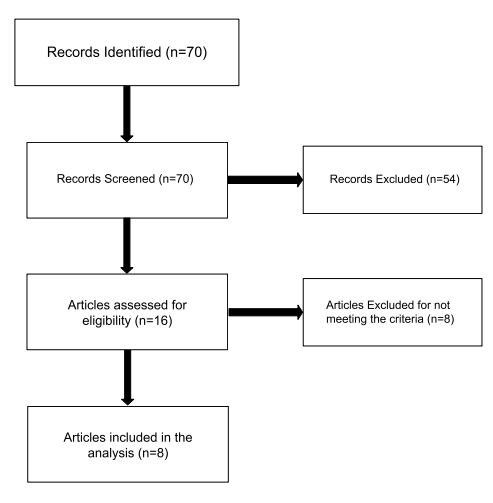
\includegraphics[width=0.42\textwidth]{figs/scopus.png} 
    \caption{Scopus Query, Author's own}
    \label{fig:scopus_query}
\end{figure}

\subsection{Articles (?)}
\selectlanguage{english}\citet{rfc3} point out the concern of incidents involving firearms and knives due to insufficient security checks. Despite CCTVs have become prevalent, their constant surveillance demands often surpass human monitoring capabilities. The paper introduces an automated weapon detection system, which employs the YOLOv5 deep learning model, adapted to a carefully selected dataset. The obtained results achieved a F1 score of 0.95 when applied to CCTV footage. The study underscores the potential of neural networks and AI in enhancing real-time security measures.

\selectlanguage{english}\citet{rfc4} highlight the crucial role of establishing a secure environment in driving economic growth, especially in terms of attracting investors and tourists. While CCTV cameras remain a fundamental element in surveillance systems, their dependency on human monitoring highlights a gap in ensuring continuous vigilance. Recognizing  the challenges of real-time weapon detection, such as varied viewing angles, occlusions, and carrier concealment, the research undertakes the task of leveraging advanced, open-source deep learning algorithms to detect potential threats. A dataset was adapted by the researchers from diverse sources, including original photos, online repositories, and even film databases. Their exploration spanned several algorithms, like VGG16, Inception variants, and YOLO iterations. Through rigorous testing prioritizing precision and recall over mere accuracy, YOLOv4 emerged as the frontrunner, achieving a F1-score of 0.91 and a mean average precision of 0.92.

In their study, \selectlanguage{english}\citet{rfc5}, address the challenge of detecting concealed weapons in public spaces, despite widespread CCTV surveillance. They point out the limitations of human monitoring in effectively analyzing extensive footage. To overcome this, they develop an enhanced weapon detection system using the YOLOv5 deep learning framework, specifically trained on a dataset of 1496 images. This system excels in identifying handguns in various conditions, achieving a \ac{map} of 0.92. Additionally, their comparative analysis with YOLOv3, as shown in Figure \ref{fig:performance-Thangaraj}, indicates that YOLOv5 not only improves accuracy in handgun detection but also operates faster and with lower computational demands.

\begin{figure}[h]
    \centering 
    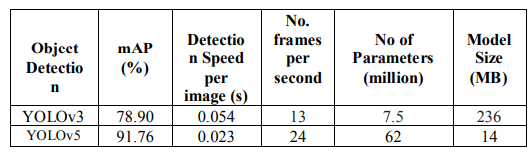
\includegraphics[width=0.55\textwidth]{figs/performance-Thangaraj.png} 
    \caption{Models Performance Comparison \selectlanguage{english}\cite{rfc5}}
    \label{fig:performance-Thangaraj}
\end{figure}

\selectlanguage{english}\citet{rfc18} refers in smart cities context the need for a advanced surveillance applied to urban security. The authors present a novel approach, combining super-resolution techniques with the YOLOv4 deep neural network, to detect knives in complex images, a task made difficult by variables like shape, size, and lighting. Their research showcases the potential of \ac{ai} surveillance to enhance real-time security, making video footage not just viewable but actionable and quantifiable. This study sets the stage for future extensions, such as firearm detection, and works as a testament to the transformative power of \ac{ai} in urban safety protocols.

\selectlanguage{english}\citet{rfc19} present an innovative security system that integrates deep learning with image processing for real-time weapon detection in CCTV feeds. The system operates by periodically capturing images from CCTV feeds and analyzing them with a convolutional neural network (CNN), enabling swift identification of potential threats. A distinctive feature of this system is the immediate notification of security personnel via a mobile app, including an image of the detected threat. The system achieves an accuracy rate of 0.92 and can detect threats within 1.6 seconds.

\selectlanguage{english}\citet{rfc17}, address the challenge of escalating urban crimes involving firearms and sharp objects in their study. They note the inadequacy of manual monitoring of the extensive data generated by omnipresent CCTVs in modern cities. To bridge this gap, they have innovated using the YOLOv8 deep learning framework, tailored to a specialized dataset including images of pistols, knives, and screwdrivers. Their system, detailed in Figure \ref{fig:safa-architecture}, goes beyond mere weapon detection; it assesses potential threat levels by analyzing the arm position of individuals holding the weapons. The system achieved 0.93 accuracy rate on CCTV footage.

\begin{figure}[h]
    \centering 
    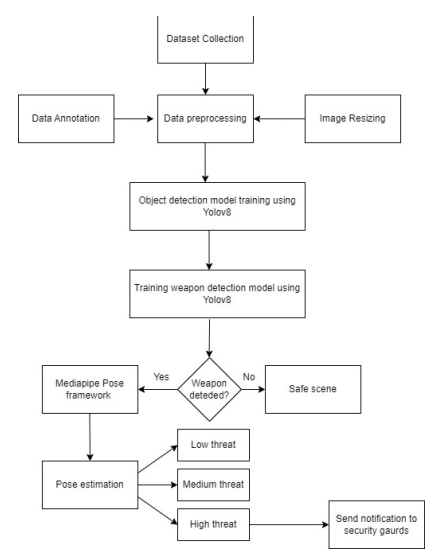
\includegraphics[width=0.55\textwidth]{figs/safa-architecture.png} 
    \caption{\selectlanguage{english}\citet{rfc17} Solution Architecture}
    \label{fig:safa-architecture}
\end{figure}


\selectlanguage{english}\citet{rfc6} research tackles the increasingly alarming scenario of weapon-related threats in crowded public spaces like banks, airports, and railway stations. Recognizing that while the deployment of CCTV cameras has seen a global surge, the sheer volume of footage can overwhelm human operators. This paper introduces a sophisticated weapon detection system, Figure \ref{fig:gawade-architecture},  that uses the power of deep learning, specifically through the use of Convolutional Neural Networks (CNN). Trained on a dataset of 10014 images, the model adeptly identifies knives, small guns, and long guns, achieving an accuracy rate of approximately 0.85.

\begin{figure}[h]
    \centering 
    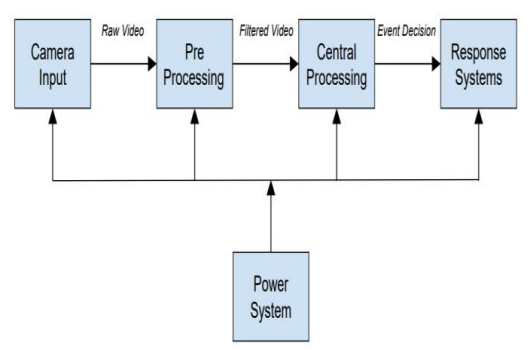
\includegraphics[width=0.55\textwidth]{figs/Gawade-architecture.png} 
    \caption{\selectlanguage{english}\citet{rfc6} Architecure Diagram}
    \label{fig:gawade-architecture}
\end{figure}

\selectlanguage{english}\citet{rfc20} address the limitations of CCTV systems, particularly their dependence on manual monitoring by police personnel, by introducing an automated weapon detection system. Utilizing two public datasets, ARMAS and IMFDB \cite{rfc28}, their research tests various object detection techniques, including SSD MobileNet-V1, EfficientDet-D0, and Faster R-CNN Inception Resnet-V2. The study highlights the effectiveness of Faster R-CNN Inception V2 with the ARMAS dataset, achieving a \ac{map} of 0.540, and \ac{ap} scores of 0.793 at 0.5 \ac{iou} and 0.627 at 0.75 IoU.

\selectlanguage{english}\citet{rfc7} emphasize the alarming rise in criminal activities in urban spaces, despite the ubiquity of CCTV systems in public areas. Recognizing the limitations of human supervision for these vast surveillance networks, they introduce an intelligent crime detection mechanism, Figure \ref{fig:shenoy-architecture}. Utilizing the SSD Mobilenet architecture fine-tuned on the DaSCI Weapon Dataset \cite{rfc29}, their solution identifies a broad spectrum of weapons, yielding an accuracy rate of 0.81. Moreover, with the integration of the GRU-based behavior analysis model, the system achieved an accuracy of 0.96 in detecting suspicious actions.

\begin{figure}[h]
    \centering 
    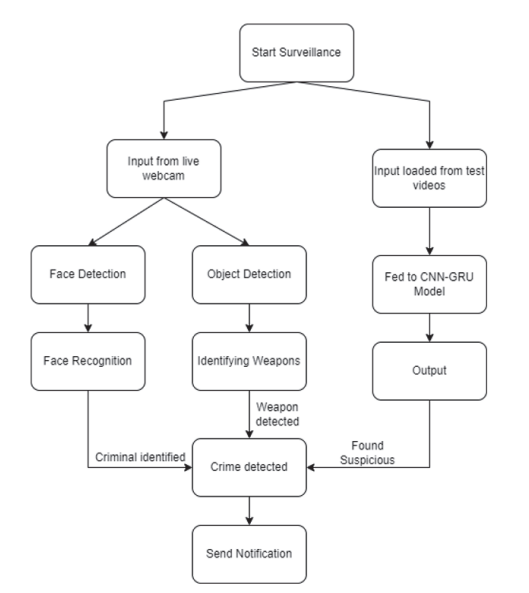
\includegraphics[width=0.6\textwidth]{figs/shenoy-architecture.png} 
    \caption{\citet{rfc7} System Architecture}
    \label{fig:shenoy-architecture}
\end{figure}

\subsection{Datasets}
In~\citet{rfc3} study, the dataset comprises three distinct classes: short guns, long guns, and knives - Figure \ref{fig:rehman-dataset}. This dataset is gathered from a variety of platforms, including surveillance videos from YouTube, simulations of firearms and knives created within the Unity framework, and images of pistols, revolvers, and knives from the Open Images Dataset as well as Kaggle. For video, a set of individual frames was extracted and manually labeled using the LabelImg Python utility. To enhance the model's training performance, data augmentation techniques were employed.

\begin{figure}[h]
    \centering 
    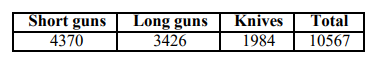
\includegraphics[width=0.45\textwidth]{figs/rheman-dataset.png} 
    \caption{Dataset images classes number~\cite{rfc3} }
    \label{fig:rehman-dataset}
\end{figure}

\selectlanguage{english}\citet{rfc4} focused on creating datasets for real-time weapon detection, specifically targeting the recognition of pistols within various environments. The data was meticulously gathered from diverse sources including the internet, YouTube CCTV videos, GitHub repositories, research groups, and the Internet Movie Firearm Database \cite{rfc28}.
They constructed three distinct datasets, being categorized into 'Pistol' and 'Not-Pistol' classes. The 'Pistol' class included pistols, revolvers, and other similar handheld weapons, while the 'Not-Pistol' class comprised objects often mistaken for weapons, such as wallets, cell phones, and metal detectors. For the data preparation and model training the researchers implemented data pre-processing steps to standardize the dataset, ensuring consistency in image size and resolution, and applied mean normalization. Also, used data augmentation strategies to artificially expand the dataset, improving the model's ability to generalize.

In the study conducted by \selectlanguage{english}\citet{rfc5}, models were trained using Google Collab~\cite{rfc26}, both Yolov3 and Yolov5, utilizing pre-trained weights on the COCO dataset~\cite{rfc16}. The dataset, comprising 1496 images, was strategically segmented into training, validation, and testing sections. Out of these, 1200 images were allocated for training, while the remaining 296 were divided for both validation and testing, each one with 148. Training a model for 40 epochs took around 120 minutes, with a standard image size set at 416x416 pixels. Both YOLOv3 and YOLOv5 were trained within the PyTorch framework. The backbone feature extraction network, used across all experiments, was pre-trained using the COCO dataset~\cite{rfc16}. Additionally, fine-tuning of the backbone was allowed during training to enhance the representation of handguns.

\selectlanguage{english}\citet{rfc6} used a comprehensive dataset consisting of 10,014 distinct weapon images to train and evaluate the model's accuracy. These images were categorized into three primary object types: knives, with a total of 3,641 images; long guns, comprising 2,497 images; and small guns, which included 3,876 images. The dataset was strategically divided, allocating 80\% of the images (8,011 images) for training and the remaining 20\% (2,003 images) for testing. Each image used had a resolution of 240 x 240 pixels, and during the training phase, they were processed in batches of 32.

\selectlanguage{english}\citet{rfc7} utilized the DaSCI Weapon Dataset \cite{rfc29} for its capability in differentiating between weapons and ordinary objects, a key feature in weapon detection. This dataset facilitated the training of the system to detect approximately 91 weapons. For the Suspicious Behavior Prediction module, the research team used the CAVIAR Dataset \cite{rfc30}, which consists of video clips depicting six different human actions. Annotations for these .mpg videos are stored in XML format, detailing both the role and context associated with each action. This information is crucial in determining whether a particular action can be classified as suspicious. To process this data, the XML file was parsed, aligning annotations with individual video frames. Each video was deconstructed frame by frame, extracting relevant data from the XML annotations. Subsequently, the data was labeled either as suspicious or not suspicious. 

\selectlanguage{english}\citet{rfc18} used two primary datasets to training and testing models related to knife detection in surveillance systems. The DaSCI Dataset \cite{rfc29} focuses on knife detection, comprising 2,078 images with various visual features of knives. The images were mainly sourced from the internet, including YouTube videos. On the other hand, the MS COCO 2017 Dataset~\cite{rfc16} is a broader computer vision dataset with 330,000 images across 80 classes. Within this dataset, 4,326 images are labeled for the 'knife' class.

\selectlanguage{english}\citet{rfc17} faced challenges in gathering a comprehensive weapon dataset, particularly for knife and screwdriver images, due to the lack of labeled datasets suitable for classifier training. To address this, they employed web scraping techniques, sourcing images from various websites and GitHub repositories. Following the collection process, manual labeling of the images was undertaken using graphical annotation tools such as LabelImg and Roboflow. The images were then preprocessed to achieve a standardized resolution of 416 x 416. The final dataset comprised approximately 6,000 images: 2,000 each of pistols, knives, and screwdrivers. For model training and testing, the images were split in an 80:20 ratio, respectively.

\selectlanguage{english}\citet{rfc19} set up a Raspberry Pi B+ and camera 1.8m high, facing a lab entrance 4.5m away to capture images of consenting students entering and exiting. To simulate potential threats, students were provided with handgun replicas, with minimal guidance on how to hold them, resulting in a variety of poses. The dataset started with 14k images at 1920p x 1080 resolution. After data augmentation like scaling and rotation, it expanded to 28k images. A challenge was the gun's small size in images, increasing misclassification risks.

\selectlanguage{english}\citet{rfc20} sourced images of firearms-related crime intentions from two primary datasets: the ARMAS Weapon Detection Dataset, which contains 3,000 clear images of pistols, some held by individuals; and the IMFDB Weapon Detection System \cite{rfc28}, which combines 4,940 diverse images of pistols and rifles from the Internet Movie Firearms Database and some CCTV footage. After collecting the data, the images were preprocessed to fit object detection training protocols and subsequently divided into training and testing subsets using an 80:20 ratio.

\section{Research Results}
\subsection{Weapon Detection Deep Learning Algorithms}
\subsection{Weapon Detection Datasets}